% $Header: /home/vedranm/bitbucket/beamer/solutions/conference-talks/conference-ornate-20min.en.tex,v 90e850259b8b 2007/01/28 20:48:30 tantau $

\documentclass[xcolor=dvipsnames]{beamer} 

\usepackage{ulem}


% This file is a solution template for:

% - Talk at a conference/colloquium.
% - Talk length is about 20min.
% - Style is ornate.



% Copyright 2004 by Till Tantau <tantau@users.sourceforge.net>.
%
% In principle, this file can be redistributed and/or modified under
% the terms of the GNU Public License, version 2.
%
% However, this file is supposed to be a template to be modified
% for your own needs. For this reason, if you use this file as a
% template and not specifically distribute it as part of a another
% package/program, I grant the extra permission to freely copy and
% modify this file as you see fit and even to delete this copyright
% notice. 


\mode<presentation>
{
  %\usetheme{boxes}
  %\usecolortheme{seagull}
  % or ...

  \setbeamercovered{transparent}
  % or whatever (possibly just delete it)

    \usecolortheme[named=OliveGreen]{structure} 
    \usetheme[height=7mm]{Rochester} 
    \setbeamertemplate{items}[ball] 
    \setbeamertemplate{blocks}[rounded][shadow=true]
}


\usepackage[czech]{babel}
% or whatever

\usepackage[utf8]{inputenc}
% or whatever

\usepackage{hyperref}
%\definecolor{links}{HTML}{2A1B81}
\hypersetup{colorlinks,linkcolor=OliveGreen,urlcolor=OliveGreen}

\usepackage{times}
\usepackage[T1]{fontenc}
% Or whatever. Note that the encoding and the font should match. If T1
% does not look nice, try deleting the line with the fontenc.


\title[Open Source] % (optional, use only with long paper titles)
{Open Source vs. INSPIRE\\INSPIRE vs. Open Source}

\subtitle {What is open source doing for INSPIRE?\\What is INSPIRE doing for
open source?}

\author[J. Čepický] % (optional, use only with lots of authors)
{Jáchym~Čepický\inst{1}\inst{2}}
% - Give the names in the same order as the appear in the paper.
% - Use the \inst{?} command only if the authors have different
%   affiliation.

\institute % (optional, but mostly needed)
{
  \inst{1}%
  Help Service - Remote Sensing s.r.o. \\
  Benešov\\
  \url{http://hsrs.cz}\\

  \inst{2}%
  OSGeo
  \url{http://osgeo.org}\\
}
  
% - Use the \inst command only if there are several affiliations.
% - Keep it simple, no one is interested in your street address.

\date[] % (optional, should be abbreviation of conference name)
{FOSS4G-CEE 2013, Bucure\c{s}ti}
% - Either use conference name or its abbreviation.
% - Not really informative to the audience, more for people (including
%   yourself) who are reading the slides online

% If you have a file called "university-logo-filename.xxx", where xxx
% is a graphic format that can be processed by latex or pdflatex,
% resp., then you can add a logo as follows:

\pgfdeclareimage[height=1.cm]{conference-logo}{imgs/conference-logo.png}
\pgfdeclareimage[height=.5cm]{hsrs-logo}{imgs/hsrs.png}
\pgfdeclareimage[height=1.0cm]{osgeo-logo}{imgs/osgeo.png}
\pgfdeclareimage[height=.5cm]{geoserver-logo}{imgs/geoserver-logo.png}
\pgfdeclareimage[height=.5cm]{pycsw-logo}{imgs/pycsw-logo.png}
\pgfdeclareimage[height=.5cm]{geon-logo}{imgs/geon-logo.png}
\pgfdeclareimage[height=.5cm]{qgis-logo}{imgs/qgis-logo.png}
\pgfdeclareimage[height=.5cm]{ol-logo}{imgs/ol-logo.png}
\pgfdeclareimage[height=.5cm]{mapserver-logo}{imgs/mapserver-logo.png}
\pgfdeclareimage[height=.5cm]{deegree-logo}{imgs/deegree-logo.png}
\pgfdeclareimage[height=.5cm]{inspire-logo}{imgs/inspire-logo.png}
%\pgfdeclareimage[height=2.0cm]{-logo}{university-logo-filename}
\logo{\pgfuseimage{conference-logo}}



% Delete this, if you do not want the table of contents to pop up at
% the beginning of each subsection:
\AtBeginSubsection[]
{
\logo{\pgfuseimage{conference-logo}}
  \begin{frame}<beamer>{TOC}
    \tableofcontents[currentsection,currentsubsection]
  \end{frame}
}


% If you wish to uncover everything in a step-wise fashion, uncomment
% the following command: 

%\beamerdefaultoverlayspecification{<+->}


\begin{document}

\begin{frame}
  \titlepage
\end{frame}

\begin{frame}{TOC}
  \tableofcontents
  % You might wish to add the option [pausesections]
\end{frame}


% Structuring a talk is a difficult task and the following structure
% may not be suitable. Here are some rules that apply for this
% solution: 

% - Exactly two or three sections (other than the summary).
% - At *most* three subsections per section.
% - Talk about 30s to 2min per frame. So there should be between about
%   15 and 30 frames, all told.

% - A conference audience is likely to know very little of what you
%   are going to talk about. So *simplify*!
% - In a 20min talk, getting the main ideas across is hard
%   enough. Leave out details, even if it means being less precise than
%   you think necessary.
% - If you omit details that are vital to the proof/implementation,
%   just say so once. Everybody will be happy with that.

\section{Openness, Open Source}

\begin{frame}{Open Source?}
  % - A title should summarize the slide in an understandable fashion
  %   for anyone how does not follow everything on the slide itself.

\begin{block}{Definition by OSI}
    The distribution terms of open-source software must comply with the following criteria: \footnote{http://opensource.org/docs/definition.html}:
    \begin{itemize} 
        \item Free redistribution 
        \item Free access to the source code
        \item Derived works
        \item \dots
    \end{itemize}
\end{block}
\end{frame}

\begin{frame}{Openness}
    
    \begin{quote}
        Open is action and conversation, not a press release or a case study. {\em[Chris Holmes]}\footnote{http://cholmes.wordpress.com/2013/05/14/opening-esri/}
    \end{quote}

    \only<1> {
        \begin{center}
            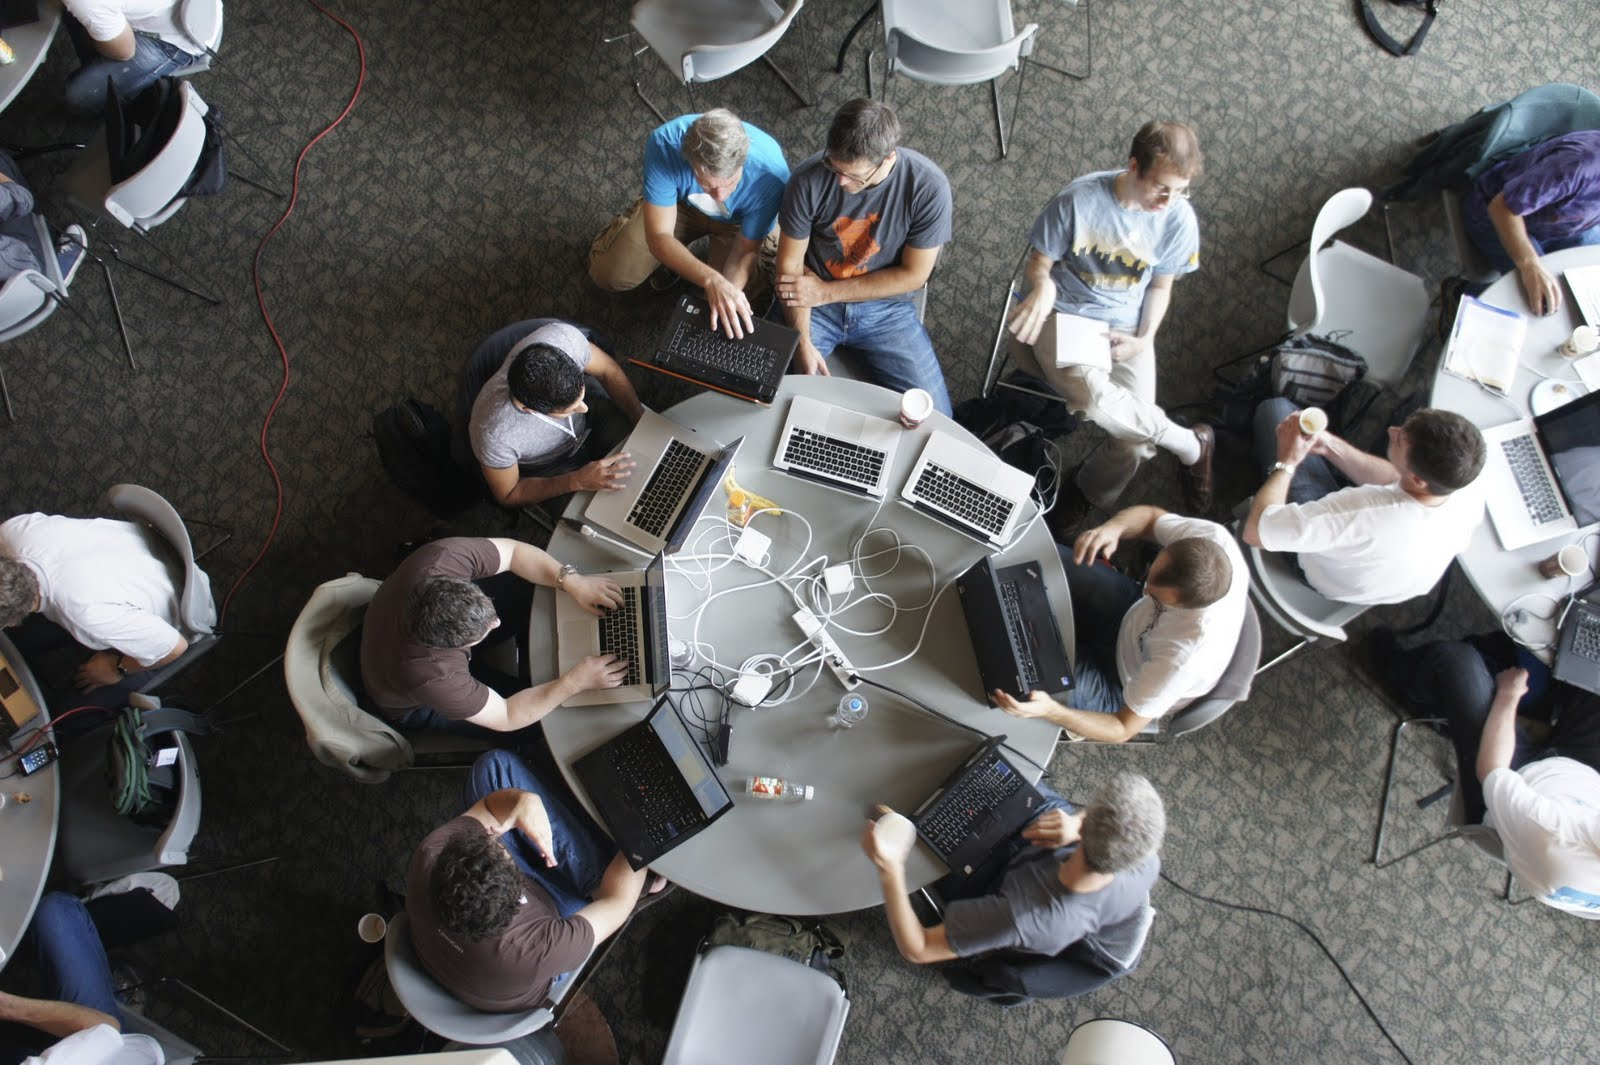
\includegraphics[width=\textheight]{imgs/ils/openess.jpg}
        \end{center}
    }
    \pause
    \only<2->{
        \begin{itemize}
            \item Prefer open standards to proprietary once 
                \pause
            \item Open you proprietary formats and services -- provide us with
                documentation
                \pause
            \item Use open forums to advocate your position, discusse with the
                community.
            \item \dots
        \end{itemize}
    }% /only
\end{frame}

\begin{frame}{Openness = freedom of movement}
        \begin{center}
            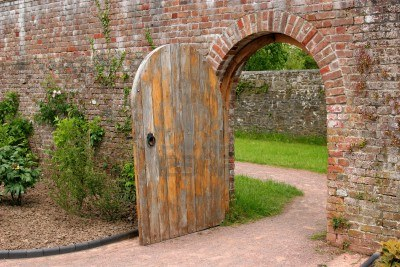
\includegraphics[width=\textheight]{imgs/ils/open-door.jpg}
        \end{center}
        
\end{frame}

\begin{frame}{Openness $=$ colaboration}
        \begin{center}
            
\includegraphics[width=\textheight]{imgs/ils/escher.jpg}
        \end{center}
\end{frame}

\begin{frame}{Openness $=$ colaboration}
    \begin{itemize}
        \item Coding (GNU/Linux, GRASS GIS, MapServer, Firefox, Chromium,
        Android, \dots)
            \pause
        \item Informations (Wikipedia)
            \pause
        \item (Geo)Data (Open Data, OpenStreetMap, OpenAerialMap, GrassRootsMapping,
        \dots)
    \end{itemize}
\end{frame}

\logo{\pgfuseimage{osgeo-logo}}
\section{Open Source Geospatial foundation}

\begin{frame}{OSGeo}
\begin{block}{Open Source Geospatial Foundation -- \href{http://osgeo.org}{OSGeo}}
\begin{quote}
    We are open source geo- community.
\end{quote}
Not-for-profit organization (US 501(c)(3) whose mission is to support the collaborative development of open source geospatial software, and promote its widespread use.

Provides financial, organizational and legal support to the broader open source geospatial community. 

It also serves as an independent legal entity to which community members can
contribute code.

{\em Project certification -- OSGeo projects}
\end{block}
\end{frame}

\begin{frame}{OSGeo Structure}
    Board of directors
    \begin{center}
    \only<1>{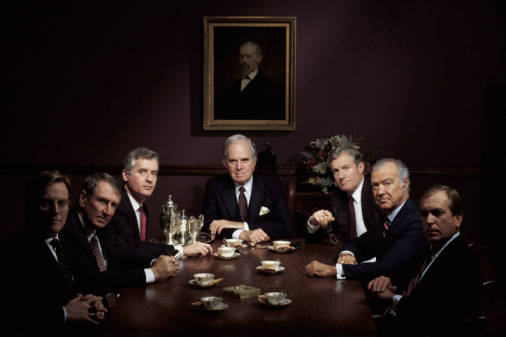
\includegraphics[height=3.5cm]{imgs/ils/board.jpg}}
    \only<2>{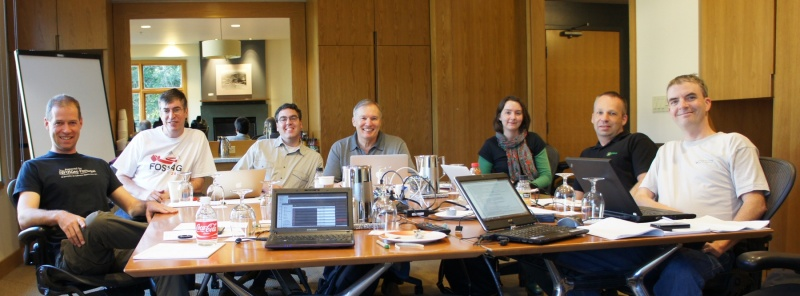
\includegraphics[height=3.5cm]{imgs/ils/osgeo-board.jpg}}
    \only<3->{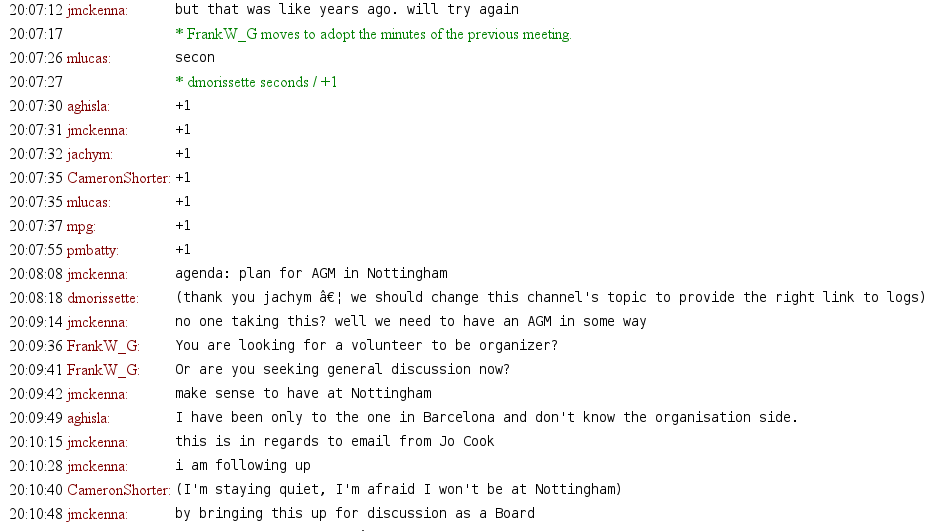
\includegraphics[height=3.5cm]{imgs/ils/osgeo-irc.png}}
    \end{center}

    \uncover<4>{
        \begin{itemize}
            \item Peter Batty, Jáchym Čepický, Michael Gerlek, Anne Ghisla, Mark Lucas,
            {\bf Jeff McKenna}, Daniel Morissette, Cameron Shorter, Frank Warmerdam
        \end{itemize}
}
\end{frame}
\begin{frame}{OSGeo Structure}
\begin{itemize}
    \item Peter Batty, Jáchym Čepický, Michael Gerlek, Anne Ghisla, Mark Lucas,
        {\bf Jeff McKenna}, Daniel Morissette, Cameron Shorter, Frank Warmerdam
    \item Charter members ($\approx$ 150) (elections!)
            \pause
        \item Local chapters (20+) (\url{http://geo-spatial.org})
            \pause
    \item Committees (Website, Finance, Incubation, {\em Education, Conference})
        \dots
\end{itemize}
\end{frame}

\logo{\pgfuseimage{inspire-logo}}
\section{INSPIRE (SDI) in OSGeo}

\begin{frame}{INSPIRE in OSGeo}
    \begin{itemize}
        \item New forming
            \href{http://wiki.osgeo.org/wiki/SDI_committee}{SDI committee}
            (focussed on INSPIRE)
        \item Current state analyzis available at
            \url{http://wiki.osgeo.org/wiki/INSPIRE} {\em } 
    \end{itemize}
\end{frame}

\subsection{View services}
\logo{\pgfuseimage{osgeo-logo}}
\begin{frame}{View services -- Server}
    \begin{itemize}
        \item \href{http://mapserver.org}{MapServer}
        \item \href{http://geoserver.org}{GeoServer}
        \item \href{http://deegree.org}{deegree}
        \item \href{http://mapguide.osgeo.org}{MapGuide}
    \end{itemize}
    \begin{flushright} 
\includegraphics[width=2cm]{imgs/ils/done.jpg} \end{flushright} 
\end{frame}

\begin{frame}{View services -- Client}
    \begin{itemize}
        \item \href{http://openlayers.org}{OpenLayers}
        \item \href{http://qgis.org}{QGIS}
    \end{itemize}
    \begin{flushright} 
\includegraphics[width=2cm]{imgs/ils/done.jpg} \end{flushright}
\end{frame}

\subsection{Discovery services}
\logo{\pgfuseimage{osgeo-logo}}
\begin{frame}{Discovery services}
    \begin{itemize}
        \item \href{http://geonetwork-opensource.org}{GeoNetwork}
        \item \href{http://deegree.org}{deegree}
        \item \href{http://pycsw.org}{pycsw}
    \end{itemize}
    \begin{flushright} 
\includegraphics[width=2cm]{imgs/ils/done.jpg} \end{flushright}
\end{frame}

\subsection{Download services}
\logo{\pgfuseimage{osgeo-logo}}
\begin{frame}{Stahovací služby}
    \begin{itemize}
        \item \href{http://geoserver.org}{GeoServer}
        \item \href{http://mapserver.org}{MapServer}
        \item \href{http://deegree.org}{deegree}
    \end{itemize}
    \begin{flushright}
\includegraphics[width=2cm]{imgs/ils/done.jpg}\end{flushright}
\end{frame}


\subsection{Work must go on}
\begin{frame}{Work must go on}
    \begin{center} 
        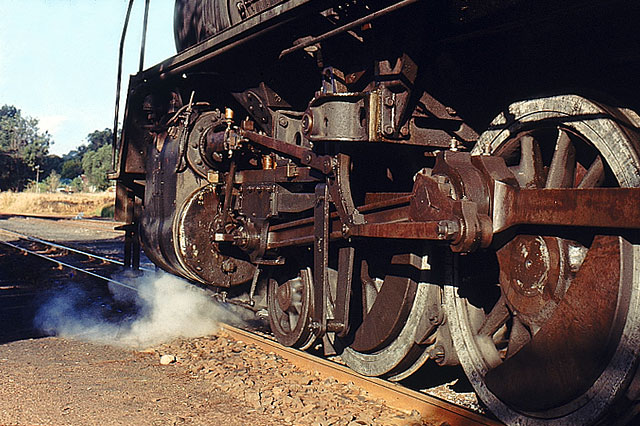
\includegraphics[width=\textwidth]{imgs/ils/engine.jpg}
    \end{center}
\end{frame}

\logo{\pgfuseimage{mapserver-logo}}

\begin{frame}{MapServer}
    INSPIRE-related documentation
    \url{http://mapserver.org/ogc/inspire.html}. 

\begin{itemize}
    \item 6.0.3 (May 2012)
        \begin{itemize}
            \item WCS axis order and other fixes
            \item Fixed resolution when UoM changes in WCS 2.0
            \item Fixed OWS GetCapabilities to report only requests/operations that are enabled.
            \item \dots
        \end{itemize}
        \pause
    \item 6.2.0 (November 2012)
        \begin{itemize}
            \item INSPIRE View Service compliant, i.e. supports the provision of an INSPIRE View Service compliant WMS Server.
        \end{itemize}
        \pause
    \item 6.2.1 (April 2013)
        \begin{itemize}
            \item GetCapabilities fixes
        \end{itemize}
\end{itemize}
\end{frame}

\logo{\pgfuseimage{geoserver-logo}}
\begin{frame}{GeoServer}
    GeoSolutions: \href{http://slideshare.net}{Analysing GeoServer compatibility with INSPIRE requirements}.
Since 2.1.0 INSPIRE plugin
    \begin{itemize}
        \item 2.1.4 (June 2012)
            \pause
        \item 2.2.2 (October 2012) Fix for INSPIRE plugin and GetFetureInfo
            \pause
        \item 2.2.5 (February 2013) Fix for WMS GetLegendGraphic, fix of pixel
            size by WCS
            \pause
        \item 2.3.0 (Marz 2013) Fixies of WCS 2.0.0, \dots
            \pause
        \item 2.3.2 (May 2013) INSPIRE community plugin became official
            GeoServer extension
    \end{itemize}
\end{frame}

%\begin{frame}{GeoServer}
%\begin{itemize}
%    \item View Services
%    \begin{itemize}
%        \item Podpora pro WMS 1.3, upravená metadata GetCapabilies, 
%        \item Podpora pro multi-jazyčné popisy
%        \item Podpora požadovaných souř. systémů a formátů
%        \item Podpora pro SLD
%    \end{itemize}
%    \pause
%    \item Download service
%    \begin{itemize}
%        \item GML 3.2.1
%        \item \dots
%    \end{itemize}
%\end{itemize}
%\end{frame}

\logo{\pgfuseimage{deegree-logo}}
\begin{frame}{deegree}
    \href{http://deegree.org}{Deegree} build and tested in Germany (Bonn).
    Deegree was choosen for the main INSPIRE geoportal.

More info about deegree a INSPIRE at
\url{http://wiki.deegree.org/deegreeWiki/InspireNode}

3.2.0-3.2.3 (March - April 2013) -- Fixes for INSPIRE download service and View service
\end{frame}

\logo{\pgfuseimage{geon-logo}}
\begin{frame}{GeoNetwork}
Two years of work between 2.6 a 2.8.
    \begin{itemize}
        \item Custom parameters to CSW request
        \item Versioning of metadata
        \item GeoServer interface
        \item \dots (mor than 500 changes)
    \end{itemize}
\end{frame}

\logo{\pgfuseimage{pycsw-logo}}
\begin{frame}{PyCSW}
    \href{http://pycsw.org}{PyCSW} relatively new project (2011), OSGeo
    incubation. 
    \begin{itemize}
        \item OGC compliant CSW and Reference Implementation since 1.4.0
        \item Implements the INSPIRE Discovery Service Technical Guidance v 3.0
since version 1.0.0
        \item No UI
        \item New release 2013-6, fix ISO metadata parser for dealing with non
            existing elements, \dots
        % \item Referenční implementace OSGeo
    \end{itemize}
\end{frame}

\logo{\pgfuseimage{qgis-logo}}
\begin{frame}{QGIS}
\sout{Desktop} \sout{(geo)data viewer} \sout{full featured} GIS Platform . Contains WMS, WFS
    clients, data editing.
    INSPIRE modules:
    \begin{itemize}
        \item Atom client (INSPIRE Download service 3.0)
        \item WFS 2.0 client
        \item qgCSW - CSW metadata client klient
        \item \dots
    \end{itemize}
\end{frame}

\logo{\pgfuseimage{ol-logo}}
\begin{frame}{OpenLayers}
    \href{http://openlayers.org}{OpenLayers} Web mapping framework, used in
    various projects (\href{http://hslayers.org}{HSLayers},
    \href{http://geoext.org}{GeoExt}, InterGraph Geoportal, \dots)

    \begin{itemize}
        \item Used for INSPIRE view, download and transformation service
        \item Aligned with requirements on INSPIRE data viewers.
    \end{itemize}

\end{frame}

\logo{\pgfuseimage{conference-logo}}
\section{Open source and INSPIRE}
\begin{frame}{INSPIRE and open source}
    \LARGE{TODO}
\end{frame}

\begin{frame}{INSPIRE and open source}
    \begin{itemize}
        \item INSPIRE is about data sharing, but not about data opening
            \pause
        \item INSPIRE is community, OSGeo is community -- building bridges
            \pause
        \item  Paul Smith, Robin Smith and Peter Baumann, \dots: Welcome
            to OSGeo community
            \pause
        \item  INSPIRE {\bf is} considered as opportunity to OSGeo projects
            \pause
        \item Common keywords: \#interoperability, \#openness, \#collaboration,
            \#community, \dots
            \pause
        \item Current standards, interoperability, development (WMTS, EPSG:3857,
            KLM, \dots), but {\em Walking on the water and writing software
            against standard is easy, when both are frozen}
            \pause
        \item \url{http://tinyurl.com/are3na1}
    \end{itemize}
\end{frame}

\begin{frame}{OSGeo and INSPIRE}

    %\begin{block}{Brian Timoney}
    %    Map Portals Don’t Work
    %\end{block}
    %\pause

    %\begin{block}{Chris Helm}
    %    Map Portals do work, we are just doing it wrong.
    %\end{block}
    %\pause

    Report about OSGeo appearance INSPIRE Conference 2013:
    \begin{itemize}
        \item Paper not accepted
        \pause
        \item OSGeo workshop nearly merged with another workshop
        \pause
        \item \sout{Very few people, who indicated they will help with paper and
            workshop preparation are actually going to the conference.}
            \url{http://wiki.osgeo.org/wiki/INSPIRE_conference_2013}
        \pause
        \item \sout{OSGeo people are talking about INSPIRE, but INSPIRE is not talking
            about open source}
    \end{itemize}
    \pause

    \begin{block}{Cameron Shorter}
        The biggest good of OSGeo is the community
    \end{block}


\end{frame}




\logo{\pgfuseimage{hsrs-logo}}
\section*{Conclusion}

\begin{frame}{Conclusion}

  % Keep the summary *very short*.
  \begin{itemize}
  \item
    OSGeo projects are doing their best, so they can be used inside any SDI
    \pause
  \item
    From the viewpoint of OSGeo, INSPIRE is one of key initiatives. All projects
    are implementing changes, required by INSPIRE.
    \pause
  \item 
      Open source is not the only right way. It is just another right way --
      Open source software can even be {\em professional} and {\em commercial},
      but it will always remain \alert{open}.

\begin{center} 
    
\includegraphics[height=4.5cm]{imgs/ils/oneway.png}
\end{center}
  
\end{itemize}
  
\end{frame}


\begin{frame}
    \begin{center}
        Jáchym Čepický\footnote{\url{http://les-ejk.cz}} \\
        jachym@hsrs.cz \\
        \url{http://hsrs.cz/} \\
        \url{http://osgeo.org}
    \end{center}
\end{frame}

\end{document}


